% ----------------------------------------------------------
\chapter{Algoritmos e estruturas de dados para consulta de segmentos no plano}
% ----------------------------------------------------------
Nesta seção veremos formas de construir estruturas de dados para um conjunto de segmentos no plano. Consideramos que os segmentos são fixos. Para cada estrutura construída também veremos como consultar os segmentos dentro de uma janela.

% ----------------------------------------------------------
\section{Árvore de Intervalos}
Uma árvore de intervalos é uma árvore binária onde cada nó não folha guarda um valor $v$ que representa a mediana de um conjunto de intervalos $I$. Denotaremos o conjunto de intervalos que contém o valor $v$ de $I_{mid}$. Denotaremos também o conjunto de intervalos que são menores que $v$ e não contém $v$ de $I_{esq}$, e similarmente, o conjunto de intervalos maiores que $v$ e que não o contem de $I_{dir}$. Cada nó não folha $r$ possui uma estrutura auxiliar para consultar os intervalos $I_{mid}$. A Figura \ref{fig:19} ilustra uma árvore de intervalos.
 
\subsection{Árvore de Intervalos unidimensional}
A construção considera um dado conjunto de intervalos $I$ e pode ser feita da seguinte forma. Temos os intervalos da forma $i = [x,x']$. Ao iniciar a construção, calculamos o valor da mediana, $x_{mid}$, dos intervalos em $I$ e o guardamos em um nó $r$. Vamos chamar de "mais à esquerda (menor que)" o menor ponto do intervalo, e respectivamente, "mais à direita (maior que)" o maior ponto do intervalo. Criamos três subconjuntos $I_{esq}$ e $I_{dir}$ tal que $I_{esq} = \{[x, x'] \in I : x' < x_{mid} \}$, $I_{dir} = \{[x, x'] \in I : x > x_{mid} \}$ e $I_{mid} = \{[x, x'] \in I : x \leq x_{mid} \leq x' \}$. Construímos duas estruturas de dados auxiliar $\tau_{esq}(r)$ com todos os intervalos de $I_{mid}$ ordenada considerando o ponto mais à esquerda de cada intervalo e $\tau_{dir}(r)$ considerando o ponto mais à direita do intervalo.Por fim associamos ambas  $\tau_{esq}(r)$  e  $\tau_{dir}(r)$ ao nó $r$. O processo continua de forma recursiva sobre os dois novos conjuntos $I_{esq}$ e $I_{dir}$. 

Vamos considerar o seguinte conjunto de intervalos da Figura \ref{fig:18} para ilustrar a construção de uma árvore de intervalos.

\begin{figure}[h!]
    \begin{center}
        \includegraphics[scale=1.5]{images/interval_tree5.pdf}
    \end{center}
    \caption {— Conjuntos de Intervalos na reta real}
    \label{fig:18}
\end{figure}

\begin{algorithm}[h!]
    \caption{Recebe um conjunto de intervalos $I$ na reta real. Devolve a raiz de uma árvore de intervalos.}
    \begin{algorithmic}[1]
        \Function{ConstróiÁrvoreDeIntervalos}{$I$}
            \If{$I$ for vazio}
                \Return nó folha vazio
            \Else
                \State Crie um nó $r$
                \State Faça uma ordenação sobre $I$ pelo ponto mais à esquerda
                \State Calcule $x_{mid}$ e guarde em $r$ 
                \State Calcule $I_{mid}$ construa duas listas ordenadas para $I_{mid}$
                \State $\tau_{esq}(r)$ ordenado pelo ponto mais à esquerda dos intervalos
                \State $\tau_{dir}(r)$ ordenado pelo ponto mais à direita dos intervalos
                \State Guarde $\tau_{esq}(r)$ e $\tau_{dir}(r)$ no nó $r$
                
                \State Cria os nós $r_{esquerda}$ e $r_{direita}$
                \State $r_{esquerda} \leftarrow $ \Call{ConstróiÁrvoreDeIntervalos}{$I_{esq}$}
                \State $r_{direita} \leftarrow $ \Call{ConstróiÁrvoreDeIntervalos}{$I_{dir}$}
                \State \Return $r$
            \EndIf
        \EndFunction
    \end{algorithmic}
\end{algorithm}


Vamos seguir alguns passos da construção de uma árvore de intervalos como \cite{cgi1}. Considerando os intervalos da Figura \ref{fig:19} inicialmente vamos ordenar os intervalos de $I$ pelo ponto mais à esquerda: $s_1 = [0, 7]$, $s_2 = [1, 4]$, $s_3 = [5, 12]$, $s_4 = [11,16]$, $s_5 = [14, 24]$, $s_6 = [17, 22]$, $s_7 = [19, 23]$. Criamos um nó raiz $r$ e nele armazenamos o valor da $x_{mid}  = 14$. Dividimos o conjunto de intervalos em três subconjuntos: $I_{esq}$ com os segmentos $\{s_1, s_2\}$, $I_{dir}$ com os segmentos $\{s_6, s_7\}$ por fim $I_{mid}$ com os segmentos que contem $x_{mid}$ $\{ s_3, s_4, s_5\}$. Com relação a $I_{mid}$ construímos duas listas: $\tau_{esq}(r)$ com os intervalos ordenados pelos pontos mais à esquerda $\{s_3,s_4,s_5\}$, e $\tau_{dir}(r)$ com os intervalos ordenados pelos pontos mais à direita de forma decrescente $\{s_5, s_3, s_4\}$. A subárvore à esquerda será uma árvore de intervalos sobre $I_{esq}$; e a subárvore à direita será uma árvore de intervalos sobre $I_{dir}$.Este procedimento é repetido até que o conjunto de intervalos não tenha mais nenhum intervalo. Neste caso criamos um nó folha vazio.
A Figura \ref{fig:19} ilustra a árvore de intervalos construída.

\begin{figure}[h!]
    \begin{center}
        \includegraphics[scale=1.5]{images/interval_tree1.pdf}
    \end{center}
    \caption {— Árvore de Intervalos construída}
    \label{fig:19}
\end{figure}

\subsection{Consulta de ponto em árvores de intervalo}
Seja uma árvore binária de intervalos $r$. Uma consulta nesta árvore é tal que queremos todos os intervalos que contenham o valor $q_x$ consultado.
Dado o valor $q_x$ da consulta realizamos o seguinte algoritmo: Inicialmente checamos se $q_x < r$; Caso seja, consultaremos a lista auxiliar $\tau_{esq}(r)$ e retornamos todos os intervalos que contenham $q_x$; então fazemos recursivamente a consulta passando o $r_{esquerda}$. Similarmente, caso $q_x \geq r $  consultaremos a lista auxiliar $\tau_{dir}(r)$ retornando os intervalos que contenham $q_x$ e recursivamente consultando passando $r_{direita}$.

\begin{figure}[h!]
    \begin{center}
        \includegraphics[scale=1.5]{images/interval_tree_query.pdf}
    \end{center}
    \caption{ — Consulta de um valor $q_x$ em um intervalo $[x, x']$}
    \label{fig:20}
\end{figure}


Segue o algoritmo que recebe como parâmetros a raiz de uma árvore de intervalos $r$ e ponto para consulta $q_x$.

\begin{algorithm}[h!]
    \caption{Recebe a raiz de uma árvore de intervalos $r$ e um ponto de consulta $q_x$. Devolve todos os segmentos que contem $q_x$.}
    \begin{algorithmic}[1]
        \Function{ConsultaÁrvoreDeIntervalos}{$r$, $q_x$}
            \If{$r$ não for folha}
                \If{$q_x$ for < $r$}
                    \State Consulte $\tau_{esq}(r)$ começando pelo intervalo com o ponto mais à esquerda
                    \State Reporte todos intervalos que contenham $q_x$
                    \State Pare a consulta no primeiro intervalo que não contenha $q_x$
                    \State \Call{ConsultaÁrvoreDeIntervalos}{$r_{esq}$, $q_x$}
                \Else
                    \State Consulte $\tau_{dir}(r)$ começando pelo intervalo com o ponto mais à direita
                    \State Reporte todos intervalos que contenham $q_x$
                    \State Pare a consulta no primeiro intervalo que não contenha $q_x$
                    \State \Call{ConsultaÁrvoreDeIntervalos}{$r_{dir}$, $q_x$}
                \EndIf
            \EndIf
        \EndFunction
    \end{algorithmic}
\end{algorithm}

Vamos acompanhar uma consulta na árvore construída da Figura \ref{fig:19}. Considere um ponto de consulta $q_x=1$. Iniciamos no $nó_{14}$. Como o nó não é folha, checamos se valor $q_x$ é menor que o $x_{mid}$ salvo. O $x_{mid}$ salvo é $14$, logo o ponto de consulta está à esquerda do $nó_{14}$. Consultamos $\tau_{esq}(nó_{14})$ e o intervalo $s_3$ não contem $q_x = 1$, portanto paramos a consulta em $\tau_{esq}(nó_{14})$. Então procedemos com a consulta no nó à esquerda. Note que ambos $q_x=1 \geq 1$ então consultaremos a lista $\tau_{dir}(r)$; reportando ambos $[s_1,s_2]$ que contem 1.

\subsection{Árvore de Intervalos para consulta de segmentos no plano}

Seja $S$ o conjunto de $n$ segmentos no plano $P$ paralelos aos eixos de consulta. Para consultar quais segmentos de forma $s=(s_x,s_y)(s_x', s_y)$ estão dentro de uma janela de consulta $J = [x, x'] \times [y, y']$ podemos utilizar a estrutura de dados construída no capitulo \ref{cap:desenvolvimento}, as árvores de alcance, para encontrar quais dos $2n$ pontos extremos dos segmentos estão dentro da janela $J$.Contudo essa consulta não conseguiria encontrar segmentos que cruzam a janela, isto é, ambos pontos extremos estão fora da janela, porem passam por ela.

\begin{figure}[h!]
    \begin{center}
        \includegraphics{images/interval_tree7.pdf}
    \end{center}
    \caption{ — Em azul: os segmentos encontrados pela árvore de alcance cujos pontos extremos estão dentro da janela. Em verde: os segmentos que cruzam as extremidades da janela porem não reportados pela árvore. Em cinza, os segmentos que não devem ser reportados. Em vermelho : A janela de consulta}
    \label{fig:21}
\end{figure}

Para os segmentos que cruzam a janela utilizaremos uma árvore de intervalos. Contudo, para uma consulta no plano, ela será modificada para que leve em consideração o comportamento bidimensional da consulta. Para isso adaptaremos as estruturas auxiliares $\tau_{esq}(r)$ e $\tau_{dir}(r)$.
Iremos montar o caso dos segmentos horizontais. Os verticais são análogos; porem, na orientação vertical. Um segmento $s= (s_x,s_y), (s_x',s_y)$ que cruza as duas extremidades da janela $[x, x'] \times [y, y']$, o segmento tem seu ponto à esquerda de $x$, isto é, $s_x < x$ e similarmente seu ponto mais à direita tem seu ponto depois da consulta $s_x' > x'$. Portanto, para saber se um segmento cruza a janela podemos escolher uma das extremidades da janela e fazer uma consulta para saber se o intervalo $[s_x, s_x']$ contem uma das extremidades da janela. Neste trabalho implementamos como \cite{cgi1} e consideramos a extremidade mais à esquerda da janela para consultas horizontais. E a extremidade inferior da janela para consultas verticais.
\begin{figure}[h]
\centering
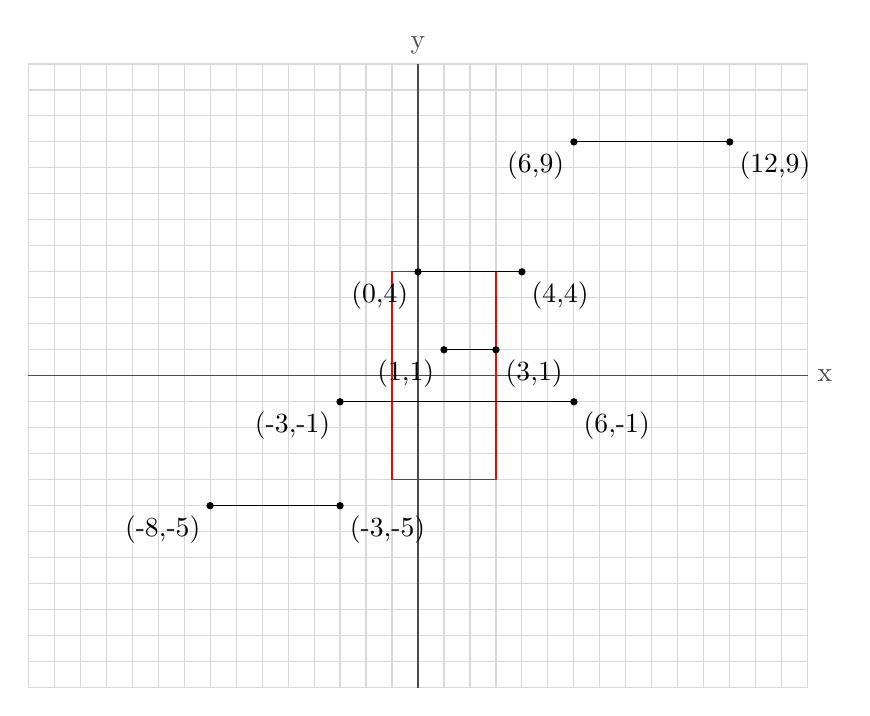
\begin{tikzpicture}[scale=0.33]
    \draw[gray!30] (-15,-12) grid[xstep=1, ystep=1]  (15,12);
    \draw[black!70] (-15,0)--(15,0) node[right]{x}; % x axis
    \draw[black!70] (0,-12)--(0,12) node[above]{y}; % y axis
    
    \draw[draw=red] (-1,4) rectangle (3,-4);

   \draw (0,4) -- (4,4);
   \draw (-8,-5) -- (-3,-5);
   \draw (6, 9) -- (12, 9);
   \draw (-3,-1) -- (6, -1);
   \draw (1,1) -- (3,1);4
   
   \fill (0,4)  circle[radius=4pt] node[anchor=north east]{(0,4)};
   \fill (4,4)  circle[radius=4pt] node[anchor=north west]{(4,4)};
   \fill (-8,-5)  circle[radius=4pt] node[anchor=north east]{(-8,-5)};
   \fill (-3,-5)  circle[radius=4pt] node[anchor=north west]{(-3,-5)};
   \fill (6,9)  circle[radius=4pt] node[anchor=north east]{(6,9)};
   \fill (12,9)  circle[radius=4pt] node[anchor=north west]{(12,9)};
   \fill (-3,-1)  circle[radius=4pt] node[anchor=north east]{(-3,-1)};
   \fill (6,-1)  circle[radius=4pt] node[anchor=north west]{(6,-1)};
   \fill (1,1)  circle[radius=4pt] node[anchor=north east]{(1,1)};
   \fill (3,1)  circle[radius=4pt] node[anchor=north west]{(3,1)};
   
\end{tikzpicture}
\caption {Em vermelho a região do retângulo de consulta}
\label{fig:23}
\end{figure}
A construção de uma árvore de intervalos para consulta de segmentos no plano é a mesma para intervalos na reta real. A diferença é a estrutura auxiliar. Ao invés de uma lista ordenada, usaremos uma árvore de alcance. Construímos uma árvore de alcance com os pontos mais à esquerda dos segmentos de $I_{mid}$ e guardamos em $\tau_{esq}$; De forma análoga construímos uma árvore de alcance com os pontos mais à direita dos segmentos de $I_{mid}$.

Vamos considerar o conjunto de segmentos no plano da Figura \ref{fig:23} para ilustrar a construção da árvore de intervalos para segmentos no plano.
Inicialmente vamos ordenar os intervalos de $I$ pelo ponto mais à esquerda: $s_1 = [(-8,-5)(-3,-5)]$, $s_2 =[(-3,-1)(6, -1)]$, $s_3 = [(0,4)(4,4)]$, $s_4 =[(1,1)(3,1)]$, $s_5 = [(6,9)(12,9)]$. Criamos um nó raiz $r$ e nele armazenamos o valor da $x_{mid}  = 1$. Dividimos o conjunto de intervalos em três subconjuntos: $I_{esq}$ com o segmento $\{s_1\}$, $I_{dir}$ com o segmento $\{s_5\}$ por fim $I_{mid}$ com os segmentos, que contem $x_{mid}$, $\{ s_2, s_3, s_4\}$. Construímos uma árvore de alcance com os segmentos de $I_{mid}$ em relação aos pontos mais à esquerda dos segmentos e associamos esta árvore a $\tau_{esq}(r)$. Construímos outra árvore de alcance com os segmentos de $I_{mid}$ considerando os pontos mais à direita e associamos a $\tau_{dir}(r)$. A subárvore à esquerda será uma árvore de intervalos sobre $I_{esq}$; e a subárvore à direita será uma árvore de intervalos sobre $I_{dir}$. A seguir a Figura \ref{fig:24} ilustra a árvore de intervalos construída.

\begin{figure}[h!]
    \begin{center}
        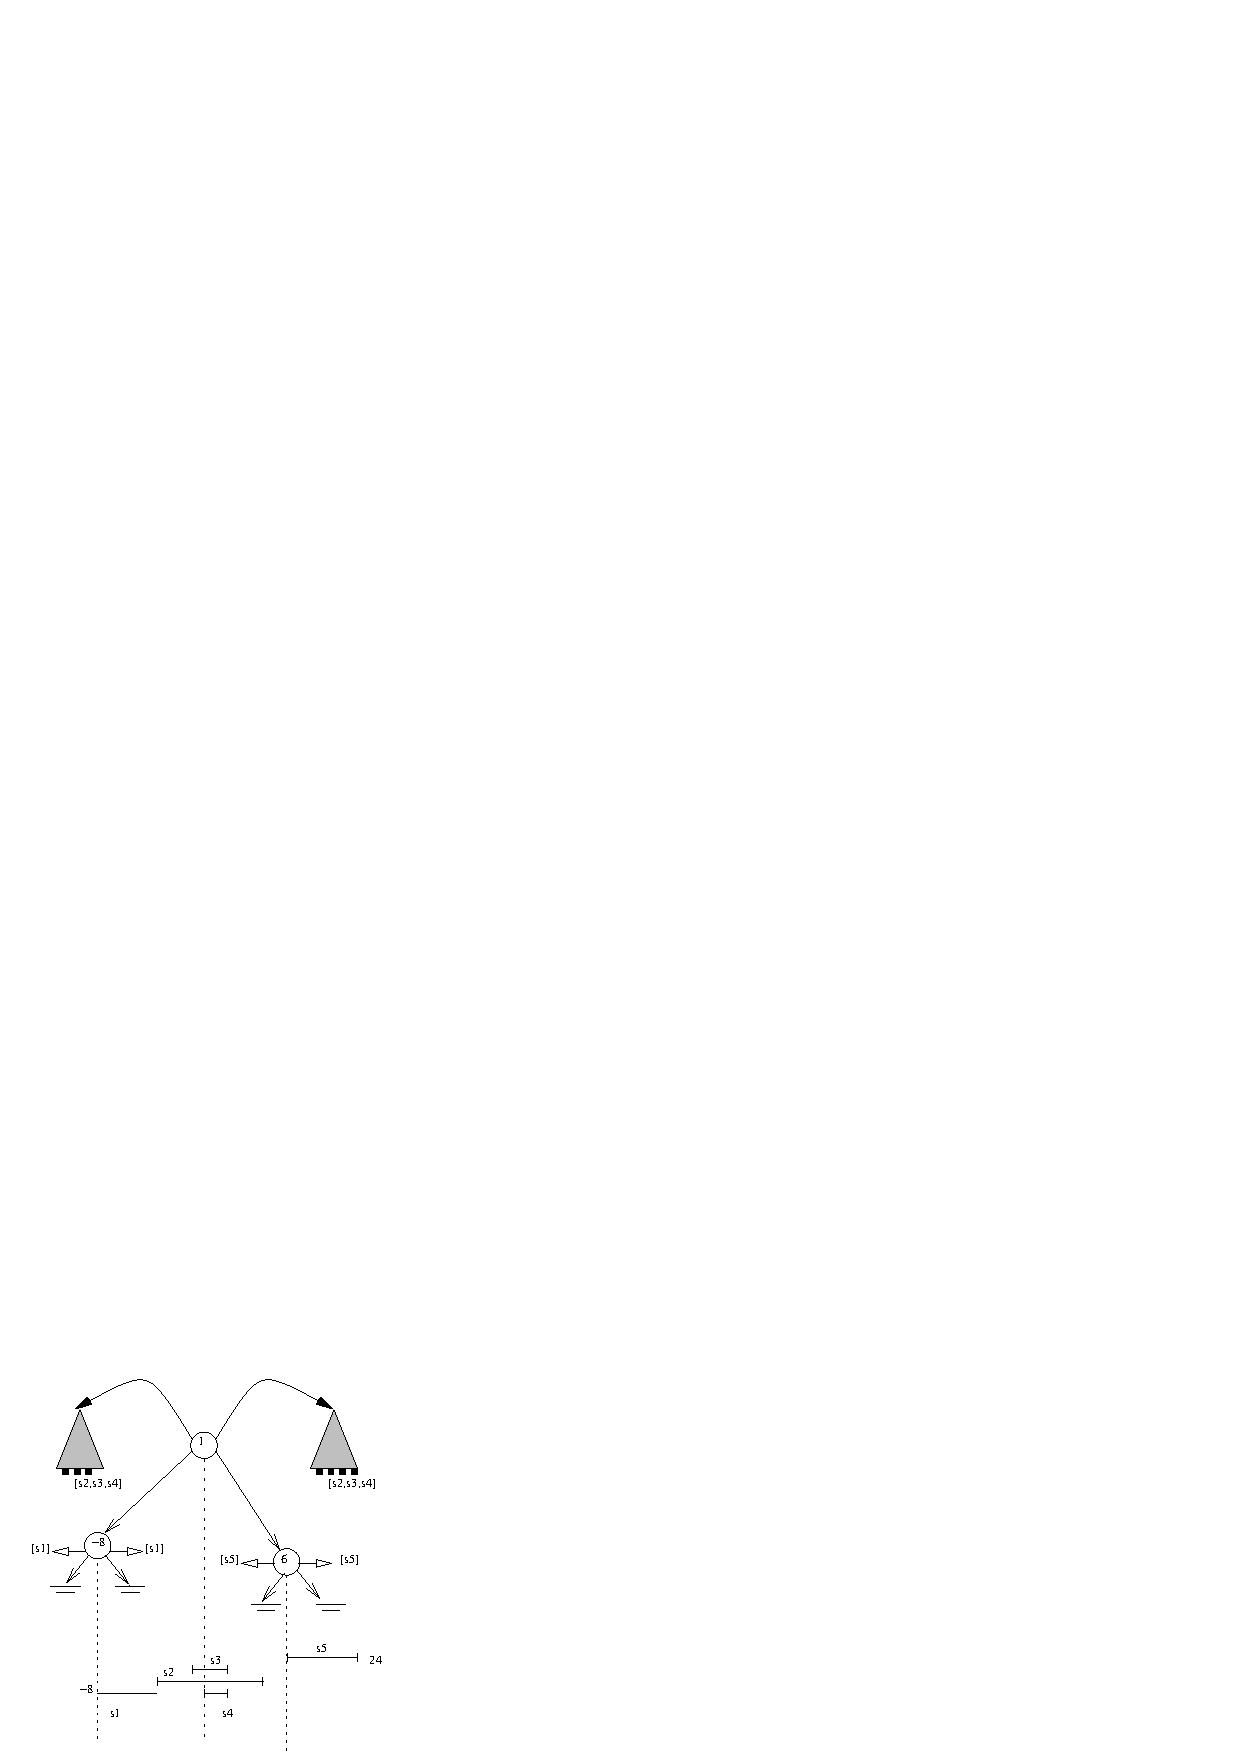
\includegraphics[scale=1.5]{images/interval_tree9.pdf}
    \end{center}
    \caption{ Árvore de intervalos construída com os segmentos da Figura \ref{fig:23}}
    \label{fig:24}
\end{figure}


\subsection{Consulta para encontrar segmentos em janela}
Uma consulta para obter os segmentos $S$  no plano que contidos em uma a janela $J=[x,x']\times[y, y']$ iremos consultar a árvore de alcance construída sobre todos os $2n$ pontos. Neste trabalho modificamos a árvore de alcance para que construa na raiz um mapa $ponto \rightarrow segmento$. Durante a consulta da árvore de alcance, está retornará todos os pontos dentro da janela e acessamos esse mapa da raiz para saber quais os intervalos associados aos pontos encontrados. Obtemos assim os segmentos que tem ao menos um ponto dentro da janela.
Para obtermos os segmentos cujos pontos extremos estão fora da janela de consulta utilizaremos a árvore de intervalos construída anteriormente.  Consultamos a estrutura auxiliar com uma janela que garante que o ponto do segmento cruza uma das laterais da janela.A consulta em $\tau_{esq}(r)$ será com a janela $J'=]-\infty, x] \times [y, y']$. Similarmente a consulta na árvore associada $\tau_{dir}(r)$  $J'=[x', \infty[ \times [y, y']$. A figura \ref{fig:fig22} ilustra essa janela de consulta. Logo depois descrevemos um algoritmo que consulta a árvore de intervalos e as estruturas associadas.

\begin{figure}[h!]
    \centering

    \tikzset{every picture/.style={line width=0.75pt}} %set default line width to 0.75pt        
    
    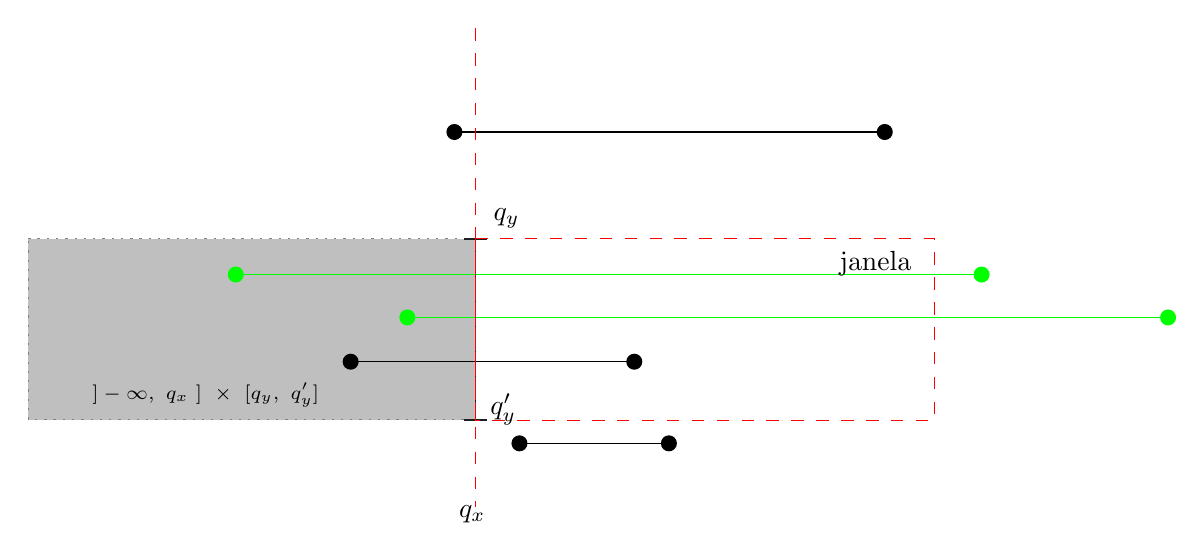
\begin{tikzpicture}[x=0.75pt,y=0.75pt,yscale=-1,xscale=1]
    %uncomment if require: \path (0,268); %set diagram left start at 0, and has height of 268
    
    %Shape: Rectangle [id:dp6848378981286898] 
    \draw  [color={gray}  ,draw opacity=1 ][fill={gray}  ,fill opacity=0.5 ][dash pattern={on 0.84pt off 2.51pt}] (56.33,111.67) -- (271.67,111.67) -- (271.67,199) -- (56.33,199) -- cycle ;
    %Straight Lines [id:da6014347269241187] 
    \draw [color={green}  ,draw opacity=1 ]   (605.5,149.67) -- (239,149.67) ;
    \draw [shift={(239,149.67)}, rotate = 180] [color={green}  ,draw opacity=1 ][fill={green}  ,fill opacity=1 ][line width=0.75]      (0, 0) circle [x radius= 3.35, y radius= 3.35]   ;
    \draw [shift={(605.5,149.67)}, rotate = 180] [color={green}  ,draw opacity=1 ][fill={green}  ,fill opacity=1 ][line width=0.75]      (0, 0) circle [x radius= 3.35, y radius= 3.35]   ;
    %Straight Lines [id:da9755427473669658] 
    \draw    (348.33,171) -- (211.67,171) ;
    \draw [shift={(211.67,171)}, rotate = 180] [color={rgb, 255:red, 0; green, 0; blue, 0 }  ][fill={rgb, 255:red, 0; green, 0; blue, 0 }  ][line width=0.75]      (0, 0) circle [x radius= 3.35, y radius= 3.35]   ;
    \draw [shift={(348.33,171)}, rotate = 180] [color={rgb, 255:red, 0; green, 0; blue, 0 }  ][fill={rgb, 255:red, 0; green, 0; blue, 0 }  ][line width=0.75]      (0, 0) circle [x radius= 3.35, y radius= 3.35]   ;
    %Straight Lines [id:da9291827808721727] 
    \draw    (365,210.33) -- (293,210.33) ;
    \draw [shift={(293,210.33)}, rotate = 180] [color={rgb, 255:red, 0; green, 0; blue, 0 }  ][fill={rgb, 255:red, 0; green, 0; blue, 0 }  ][line width=0.75]      (0, 0) circle [x radius= 3.35, y radius= 3.35]   ;
    \draw [shift={(365,210.33)}, rotate = 180] [color={rgb, 255:red, 0; green, 0; blue, 0 }  ][fill={rgb, 255:red, 0; green, 0; blue, 0 }  ][line width=0.75]      (0, 0) circle [x radius= 3.35, y radius= 3.35]   ;
    %Straight Lines [id:da8381433224809642] 
    \draw    (469,60.33) -- (261.67,60.33) ;
    \draw [shift={(261.67,60.33)}, rotate = 180] [color={rgb, 255:red, 0; green, 0; blue, 0 }  ][fill={rgb, 255:red, 0; green, 0; blue, 0 }  ][line width=0.75]      (0, 0) circle [x radius= 3.35, y radius= 3.35]   ;
    \draw [shift={(469,60.33)}, rotate = 180] [color={rgb, 255:red, 0; green, 0; blue, 0 }  ][fill={rgb, 255:red, 0; green, 0; blue, 0 }  ][line width=0.75]      (0, 0) circle [x radius= 3.35, y radius= 3.35]   ;
    %Straight Lines [id:da7444817332368282] 
    \draw [color={green}  ,draw opacity=1 ]   (515.67,129) -- (156.33,129) ;
    \draw [shift={(156.33,129)}, rotate = 180] [color={green}  ,draw opacity=1 ][fill={green}  ,fill opacity=1 ][line width=0.75]      (0, 0) circle [x radius= 3.35, y radius= 3.35]   ;
    \draw [shift={(515.67,129)}, rotate = 180] [color={green}  ,draw opacity=1 ][fill={green}  ,fill opacity=1 ][line width=0.75]      (0, 0) circle [x radius= 3.35, y radius= 3.35]   ;
    %Straight Lines [id:da4271924427932462] 
    \draw [color={rgb, 255:red, 30; green, 30; blue, 30 }  ,draw opacity=1 ]   (271.67,111.67) -- (271.67,199) ;
    \draw [shift={(271.67,199)}, rotate = 270] [color={rgb, 255:red, 30; green, 30; blue, 30 }  ,draw opacity=1 ][line width=0.75]    (0,5.59) -- (0,-5.59)   ;
    \draw [shift={(271.67,111.67)}, rotate = 270] [color={rgb, 255:red, 30; green, 30; blue, 30 }  ,draw opacity=1 ][line width=0.75]    (0,5.59) -- (0,-5.59)   ;
    %Straight Lines [id:da33530800628578705] 
    \draw [color={red },draw opacity=1 ] [dash pattern={on 4.5pt off 4.5pt}]  (271.67,10.33) -- (271.67,113.5) -- (271.67,241) ;
    %Shape: Rectangle [id:dp2955317576076706] 
    \draw  [color={red},draw opacity=1 ][dash pattern={on 4.5pt off 4.5pt}] (271.67,111.67) -- (493,111.67) -- (493,199.33) -- (271.67,199.33) -- cycle ;
    % Text Node
    \draw (262.67,239.07) node [anchor=north west][inner sep=0.75pt]    {$q_{x}$};
    % Text Node
    \draw (86,180.07) node [anchor=north west][inner sep=0.75pt]  [font=\scriptsize]  {$] -\infty ,\ q_{x} \ ] \ \times \ [ q_{y} ,\ q_{y} ']$};
    % Text Node
    \draw (279.33,96.07) node [anchor=north west][inner sep=0.75pt]    {$q_{y}$};
    % Text Node
    \draw (277.67,185.07) node [anchor=north west][inner sep=0.75pt]    {$q_{y} '$};
    % Text Node
    \draw (446,116.67) node [anchor=north west][inner sep=0.75pt]   [align=left] {janela};
    \end{tikzpicture}
    \caption{Consulta na árvore de intervalos para segmentos que cruzam a janela. Em verde os segmentos que queremos reportar com esta consulta}
    \label{fig:fig22}
\end{figure}

\begin{algorithm}[h!]
    \caption{Recebe a raiz de uma árvore de intervalos $r$ e uma janela de consulta $J=[x,x']\times[y, y']$. Devolve todos os segmentos que contem $J$.}
    \begin{algorithmic}[1]
        \Function{ConsultaÁrvoreDeIntervalosNoPlano}{$r$, $J$}
            \If{$r$ não for folha}
                \If{$q_x$ for < $r$}
                    \State Consulte \Call{Busca2DEmAlcance}{$\tau_{esq}(r)$ , $]-\infty, x] \times [y, y']$}
                    \State \Call{ConsultaÁrvoreDeIntervalosNoPlano}{$r_{esq}$, $J$}
                \Else
                    \State Consulte \Call{Busca2DEmAlcance}{$\tau_{dir}(r)$ , $[x', \infty [ \times [y, y']$}
                    \State \Call{ConsultaÁrvoreDeIntervalosNoPlano}{$r_{dir}$, $J$}
                \EndIf
            \EndIf
        \EndFunction
    \end{algorithmic}
\end{algorithm}

Vamos acompanhar uma consulta na árvore construída para a Figura \ref{fig:23}. Inicialmente queremos descobrir quais segmentos tem ao menos um ponto extremo dentro da janela. Consultamos a árvore de alcance construída com os $2n$ pontos com a janela $J=[-1,3]\times[-4,4]$. Esta consulta devolve $(1,1), (3,1), (0,4)$; consultamos o mapa na raiz da árvore e devolvemos os segmentos $[s_3, s_4]$. Seguimos para a consulta da árvore de intervalos; Iniciamos na raiz $nó_1$. Como o nó não é folha, checamos se $-1$ (a extremidade esquerda da janela) é menor que o $x_{mid}$ salvo no nó. O $x_{mid}$ salvo é 1, logo a consulta está à esquerda de $nó_1$. Consultamos a árvore associada $\tau_{esq}(nó_1)$ com a janela  $]-\infty, -1] \times [-4, 4]$ devolvendo $(-3, -1)$; utilizando o mapa associado à raiz devolvemos o segmento $[s_2]$.
A Figura \ref{fig:fig25} a seguir é a nossa implementação para consulta de segmentos horizontais no plano.

\begin{figure}[h]
\centering
\begin{minipage}{.5\textwidth}
  \centering
  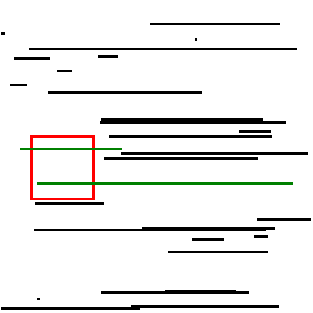
\includegraphics[width=.8\linewidth]{images/inside_segments.pdf}

  \label{fig:test1}
\end{minipage}%
\begin{minipage}{.5\textwidth}
  \centering
  
  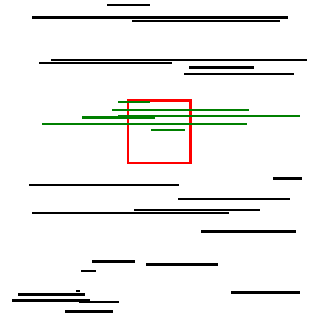
\includegraphics[width=.8\linewidth]{images/inside_segments2.pdf}
  \label{fig:test2}
 
\end{minipage}
 \caption{Resultados das consultas em janela com Árvore de Intervalos no plano}
 \label{fig:fig25}
\end{figure}